\documentclass[letterpaper,12pt]{article}

\usepackage{ucs}
\usepackage[utf8x]{inputenc}
\usepackage{amsmath}
\usepackage{amsfonts}
\usepackage{amssymb}
\usepackage[margin=1in]{geometry}
\usepackage{enumerate}
\usepackage{graphicx}

\newcommand{\abs}[1]{\lvert #1\rvert}
\newcommand{\len}[1]{\lVert #1\rVert}
\newcommand{\R}{\mathbb{R}}
\newcommand{\N}{\mathbb{N}}
\newcommand{\Z}{\mathbb{Z}}
\newcommand{\x}{\mathbf{x}}
\newcommand{\y}{\mathbf{y}}
\newcommand{\inter}[1]{\overset{\,\,\circ}{#1}}
\newcommand{\T}{\mathcal{T}}
\DeclareMathOperator{\Int}{Int}

\title{Math 4310 Assignment \#12\\University of Lethbridge, Fall 2014}
\author{Sean Fitzpatrick}
\begin{document}
 \maketitle

{\bf Due date:} Wednesday, December 3rd, by 5 pm.

\bigskip

Please submit solutions to the following problems (except where indicated). As usual, all the textbook exercises are recommended as practice problems if they don't appear as an assigned problem below.

\begin{enumerate}
\item Prove that the antipodal map $f:S^1\to S^1$ given by $f(z)=-z$ is homotopic to the identity map.

{\em Hint:} The antipodal map can be written as $f(e^{i\theta}) = f(e^{i(\theta+\pi)})$.

\item Let $f:S^1\to S^1$ be the antipodal map as above. What is the effect of the induced isomorphism
\[
f_*:\pi_1(S^1,1)\to \pi_1(S^1,-1)?
\]
\item (Do not hand in) Let $T = S^1\times S^1$ denote the two-dimensional torus. Show that there is a deformation retraction of the punctured torus $T\setminus\{p\}$ onto a pair of circles joined at a point, where $p\in T$ is any point.

Think about this one for a bit. I was going to make it a bonus except it's incredibly easy to Google the solution. So instead, think about it. Once you've thought about it, Google it. You should be able to find a nice YouTube video illustrating exactly how the retraction works.

\item Prove that the space $X = \R^2\setminus \{p,q\}$, where $p,q\in\R^2$ with $p\neq q$ is homotopy equivalent to the figure-eight space $Y$ given by joining two circles at a point $b$.
\begin{center}
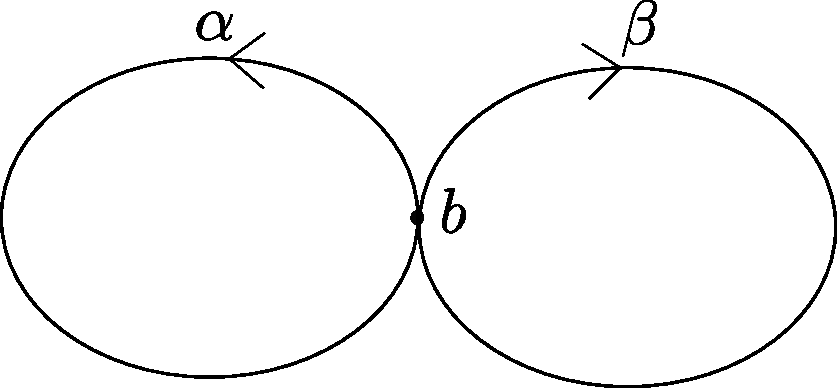
\includegraphics[width=3in]{figure8.pdf}
\end{center}

\end{enumerate}
\end{document}
 
